\textbf{COLUNI 2022 -- Questão 28}\par\medskip Leia os textos a seguir.

\par

\textbf{TEXTO I}

\begin{center}\textbf{A história da primeira vacina}\end{center} O primeiro indício de vacina surgiu na China, no século X, contra a varíola, [...] cientistas da época transformavam cascas de ferida de varíola em um pó contendo o vírus já inativo e espalhavam nos ferimentos das pessoas já contaminadas. Esse método ficou conhecido como variolação. Alguns séculos depois, em 1796 [...] Edward Jenner [...] fez um experimento e aplicou em um menino chamado James Phipps de oito anos, uma pequena dose de varíola bovina. O garoto ficou doente, mas manifestou uma forma branda da doença. Após a recuperação de James, Jenner introduziu na criança o vírus da doença humana em sua forma mais fatal, retirado de uma ordenhadeira. O menino, já imune, não desenvolveu a varíola. A palavra “vacina” vem de “vacca”, justamente pelo contexto histórico. Disponível em: https://butantan.gov.br/noticias/imunizacao-uma-descoberta-da-ciencia-que-vem-salvando-vidas-desde-o-seculo-xviii. Acesso em: 01 set. de 2021 (Adaptado).

\par

\textbf{TEXTO II}

\par

Desde que começaram a ser produzidas em massa, as vacinas se tornaram um dos principais elementos para o combate a doenças no mundo. A vacinação tem contribuído para reduzir expressivamente a incidência de pólio, sarampo e tétano, entre várias outras doenças, como exemplificado nos gráficos abaixo.

% COLUNI-AUTO-FIGURES-BEGIN
\begin{figure}[htbp]
\centering
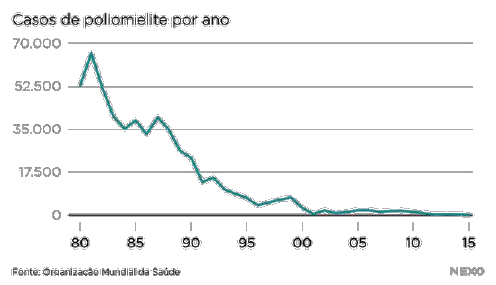
\includegraphics[width=0.95\linewidth]{static/simulados/coluni/figuras/2022/questao-28/figura-1.png}
\end{figure}
\begin{figure}[htbp]
\centering
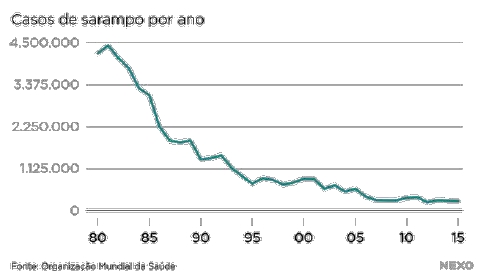
\includegraphics[width=0.95\linewidth]{static/simulados/coluni/figuras/2022/questao-28/figura-2.png}
\end{figure}
% COLUNI-AUTO-FIGURES-END

Disponível em: https://www.bio.fiocruz.br/index.php/br/noticias/1263-vacinas-as-origens-a-importancia-e-os-novos-debates-sobre-seuuso?showall=1\&limitstart=. Acesso em: 01 set. 2021 (Adaptado).

\par



\par

\textbf{TEXTO III}

\par

Com a pandemia da COVID-19, causada pelo novo coronavírus, a humanidade pôde assistir a ciência desenvolver diversas vacinas em tempo recorde. Em apenas 10 meses, algumas das vacinas listadas no quadro a seguir já haviam sido desenvolvidas, muitas delas com a utilização da Tecnologia do DNA Recombinante.

\par

\begin{center}
\begin{tabular}{l|l}
\textbf{Laboratório} & \textbf{Tecnologia Empregada} \\ \hline
Astrazeneca e Universidade de Oxford & Adenovírus Vetor \\ \hline
Sinovac e Instituto Butantan & Vírus Inativado \\ \hline
Pfizer-Wyeth & RNA \\ \hline
Janssen-Cilag & Adenovírus Vetor \\ \hline
Instituto Butantan & Vírus quimérico inativado
\end{tabular}
\end{center}

Disponível em: https://www.bbc.com/portuguese/internacional-55232520.amp. Acesso em: 13 set. 2021 (Adaptado).

\par

De acordo com os textos I, II e III e com os conhecimentos sobre vacinas, é INCORRETO afirmar que:


\begin{enumerate}
\item quando a vacina é introduzida no corpo humano, o sistema imunológico inicia a produção de anticorpos
        contra o antígeno presente na vacina e, ao final da resposta imunológica, são geradas células de memória
        que responderão rapidamente caso ocorra novo contato com o antígeno.
\item a contribuição das vacinas no controle e, até mesmo, na erradicação de várias doenças pode ocorrer de
        diversas formas, por exemplo, evitando o desenvolvimento da doença ou a gravidade dela.
\item as vacinas, produzidas ou não por meio da engenharia genética, podem prevenir ou impedir o contágio
        pelos patógenos causadores de uma doença e a transmissão deles entre os membros da população.
\item no controle de muitas doenças, deve-se somar ao desenvolvimento das vacinas e à ampla aplicação
        delas, o conhecimento e o acesso a outros métodos de prevenção e de tratamento adequados.\end{enumerate}
